% EF5342 Week 2 — Interest Rates
% Beamer conversion from week2_InterestRate.pptx (54 source slides -> 40 frames).
% Compile: pdflatex week2_InterestRate.tex
% Each frame carries a [src: ...] comment mapping back to source slides.
\documentclass[aspectratio=169]{beamer}
\usepackage{../ef5342}

\title{EF5342 Financial Systems, Markets and Instruments}
\subtitle{Week 2 --- Interest Rates}
\author{Prof.\ Weikai Li}
\institute{City University of Hong Kong}
\date{Semester B 2026--2027}

\begin{document}

% [src: 1]
\begin{frame}
\titlepage
% Source slide 1 title image (slide01_img.jpg) dropped: decorative cover art.
\end{frame}

% ============ PART I: DETERMINANTS OF INTEREST RATES ============

% [src: 2, 3]
\section{Determinants of Interest Rates}
% Roadmap (source slide 2): Determinants of Interest Rates; Term Structure of
% Interest Rates (Yield Curve); Time Value of Money.

% [src: 4, 5]
\begin{frame}{Interest Rate Basics: Nominal vs.\ Real}
\begin{description}
  \item[Nominal interest rate ($i$)] The rate actually observed in financial markets (bonds or loans)
  \item[Real risk-free rate (RFR)] The true increase in purchasing power earned on a risk-free investment
\end{description}
\vspace{0.3em}
\textbf{Fisher equation:} nominal rates contain compensation for expected inflation --- $i \approx RFR + E(IP)$, exactly $1+i = (1+RFR)(1+E(IP))$.
\vspace{0.3em}

\emph{Example:} 10-year Treasury yield 5\%, expected inflation 3\% $\Rightarrow$ RFR $\approx 5\%-3\% = 2\%$ (exact: $1.05/1.03 - 1 \approx 1.94\%$). Your money grows 5\% in dollar terms, but inflation erodes purchasing power by 3\%, so real wealth rises only $\sim$2\%.
\vspace{0.3em}

In valuation (DCF, CAPM) use the \textbf{nominal} risk-free rate with nominal cash flows; with real (inflation-adjusted) cash flows, the \textbf{real} rate is the consistent choice. Nominal = what you see and get paid; real = what matters for long-term wealth growth after inflation.
\note{RFR measures society's relative time preference for consuming today rather than tomorrow.}
\end{frame}

% [src: 6]
\begin{frame}{Nominal Interest Rate and Inflation (US, 1986--2025)}
\begin{table}
\centering
\small
\begin{tabular}{p{0.36\textwidth}p{0.08\textwidth}p{0.22\textwidth}p{0.22\textwidth}}
\toprule
\textbf{Metric} & \textbf{Mean} & \textbf{Max} & \textbf{Min} \\
\midrule
10-Year Treasury yield (nominal risk-free) & 5.1\% & 10.6\% (1986) & 0.5\% (2020) \\
CPI inflation (YoY) & 2.8\% & 8.0\% (2022) & $-0.4\%$ (2009) \\
Real risk-free rate (nominal $-$ inflation) & 2.3\% & 7.0\% (1986) & $-5.5\%$ (2022) \\
\bottomrule
\end{tabular}
\end{table}
\begin{center}
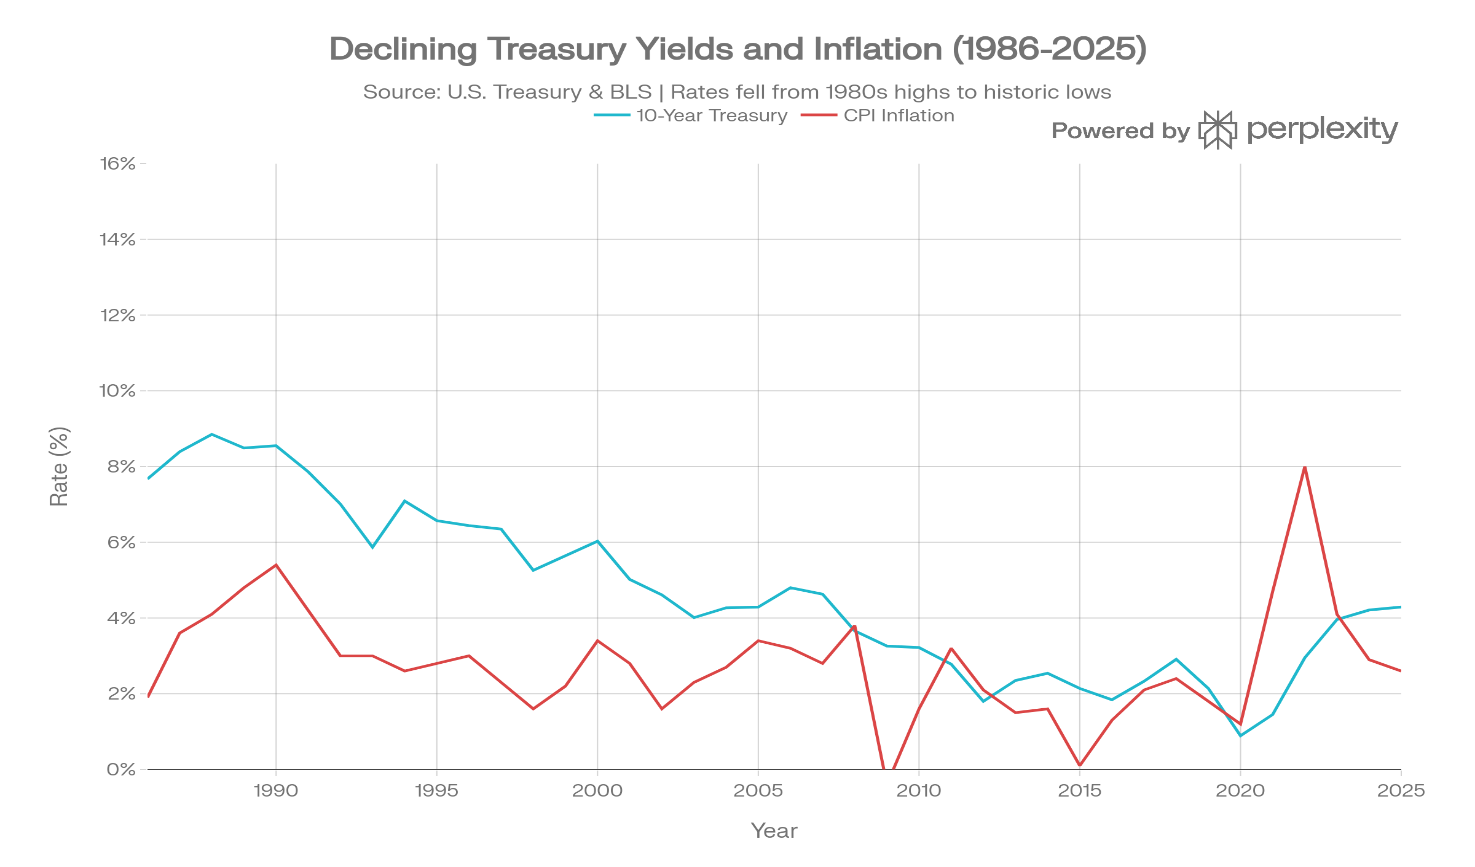
\includegraphics[width=0.46\textwidth,height=0.34\textheight,keepaspectratio]{figures/slide06_img_flat.png}
\end{center}
\begin{center}
\small Table and chart show the 1986--2025 sample; as of 8 September 2026 the 10-year Treasury yield stands at 4.79\%.
\end{center}
\end{frame}

% [src: 7]
\begin{frame}{The Real Risk-Free Rate}
The negative-rate era has ended: as of September 2026, no major central bank maintains a negative policy rate (ECB 1.50\%, BoJ 0.75\%, SNB 0.00\%). The 2020--2023 episode was historically severe --- pandemic-era monetary stimulus, supply-chain disruptions, and fiscal spending pushed inflation well above Treasury yields.
\begin{center}
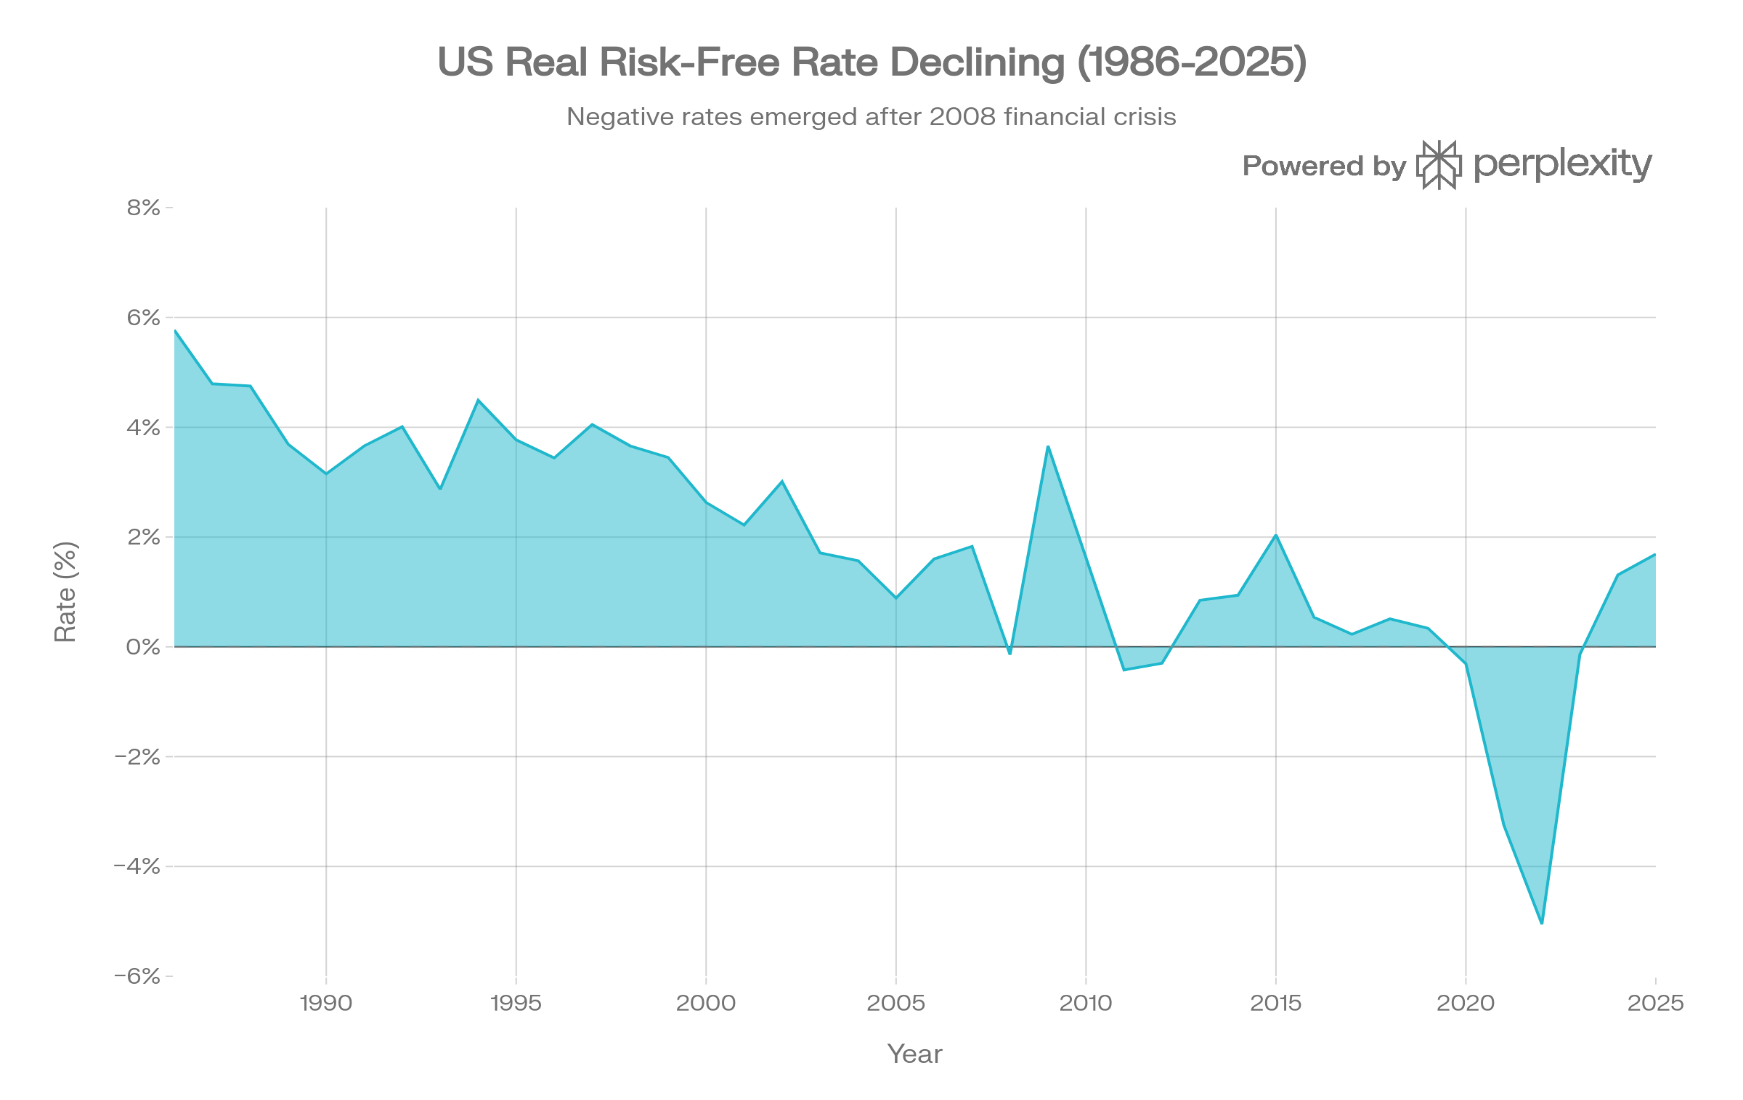
\includegraphics[height=0.60\textheight,keepaspectratio]{figures/slide07_img_flat.png}
\end{center}
\end{frame}

% [src: 8, 9]
\begin{frame}{Loanable Funds Theory}
Explains interest-rate \emph{levels} and \emph{movements}:
\begin{itemize}
  \item The level of interest rates results from the \textbf{supply of and demand for loanable funds} --- the interest rate is the \emph{price} of loanable funds
  \item Market participants --- consumers, businesses, governments, foreigners --- are categorized as net suppliers or net demanders of funds
  \item The \textbf{equilibrium rate} $i^*$ is where quantity supplied equals quantity demanded ($Q^*$)
\end{itemize}
\vspace{0.3em}
Supply slopes upward, demand slopes downward; their intersection gives $(i^*, Q^*)$.
\note{Ignore inflation for the moment. Higher interest rates induce suppliers to supply more loanable funds (higher return); higher rates reduce demand (borrowing is costlier).}
\end{frame}

% [src: 10, 11]
\begin{frame}{Supply and Demand of Loanable Funds}
\begin{columns}
\begin{column}{0.48\textwidth}
\textbf{Supply} --- mainly savings (funds not consumed today):
\begin{itemize}
  \item Household savings
  \item Business retained earnings
  \item Government budget surplus (public saving)
  \item Foreign capital inflows
\end{itemize}
\vspace{0.2em}
Upward-sloping: higher real rates $\Rightarrow$ greater incentive to save (postpone consumption) $\Rightarrow$ more funds supplied.
\end{column}
\begin{column}{0.48\textwidth}
\textbf{Demand} --- from borrowers:
\begin{itemize}
  \item Firms borrowing for physical capital (machinery, factories, R\&D) --- most important
  \item Households for big-ticket items (homes, cars)
  \item Government financing budget deficits
\end{itemize}
\vspace{0.2em}
Downward-sloping: higher real rates $\Rightarrow$ borrowing costlier $\Rightarrow$ fewer profitable projects $\Rightarrow$ less funds demanded.
\end{column}
\end{columns}
\note{Ignore inflation for the moment (both slides).}
\end{frame}

% [src: 12]
\begin{frame}{Shifts in the Curves Change Equilibrium Rates}
\begin{description}
  \item[Increased supply of loanable funds] Supply shifts right (SS $\to$ SS*) --- equilibrium moves E $\to$ E*: quantity rises ($Q^* \to Q^{**}$) and the interest rate \emph{falls} ($i^* \to i^{**}$)
  \item[Increased demand for loanable funds] Demand shifts right (DD $\to$ DD*) --- equilibrium quantity rises ($Q^* \to Q^{**}$) and the interest rate \emph{rises} ($i^* \to i^{**}$)
\end{description}
\end{frame}

% [src: 13, 14]
\begin{frame}{Key Interest Rates Over Time (US)}
The \textbf{federal funds rate} is the rate at which depository institutions lend reserve balances to other banks overnight --- the interest rate set by the Fed.
\begin{center}
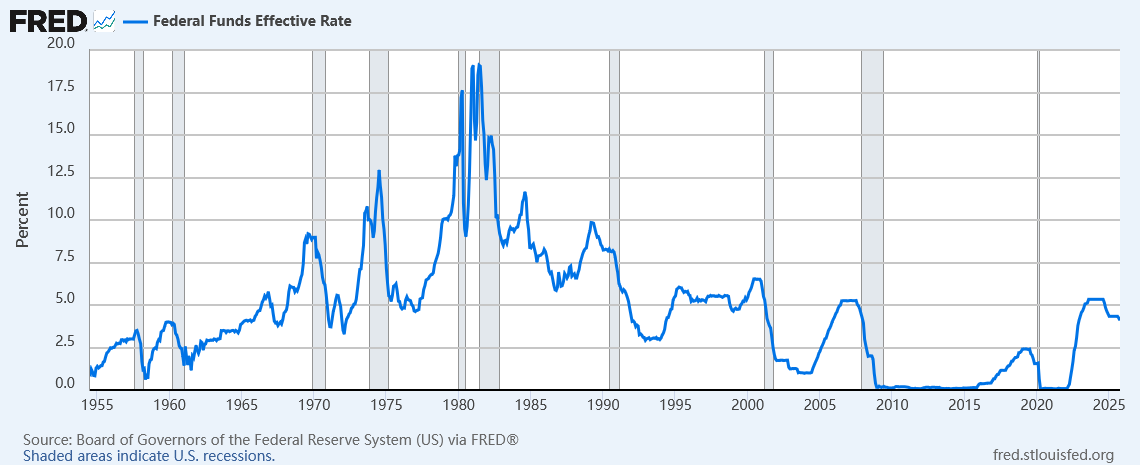
\includegraphics[height=0.62\textheight,keepaspectratio]{figures/slide13_img_flat.png}
\end{center}
\begin{center}
\small Source: Federal Reserve Bank of St.\ Louis
\end{center}
\end{frame}

% [src: 14]
\begin{frame}{Key Interest Rates Over Time (US), cont.}
\begin{figure}
\centering
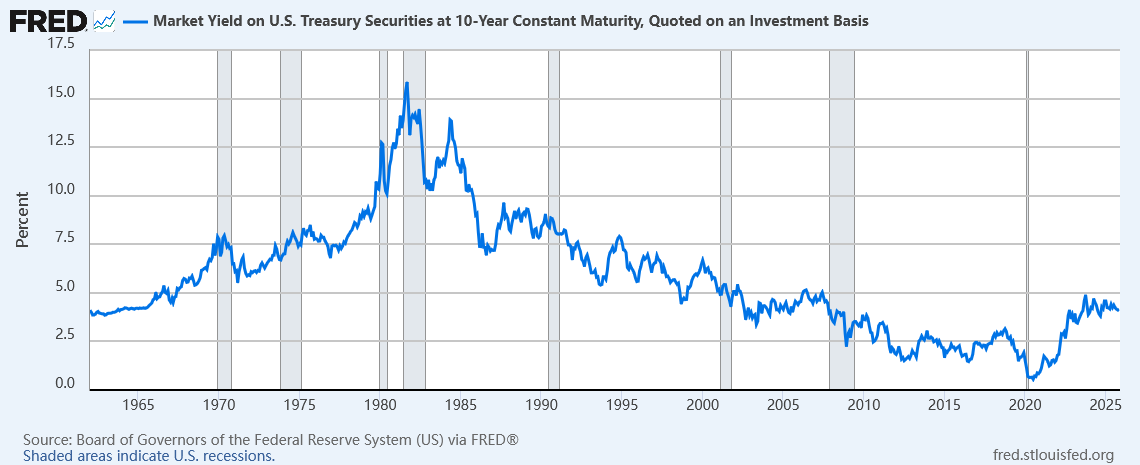
\includegraphics[height=0.70\textheight,keepaspectratio]{figures/slide14_img_flat.png}
\end{figure}
\begin{center}
\small Source: Federal Reserve Bank of St.\ Louis
\end{center}
\end{frame}

% [src: 15, 16]
\begin{frame}{Key Interest Rates in Hong Kong}
The \textbf{HIBOR} (Hong Kong Interbank Offered Rate) is the main benchmark rate at which banks offer to lend HK dollar funds to other banks in the Hong Kong interbank market.
\begin{columns}
\begin{column}{0.5\textwidth}
\centering
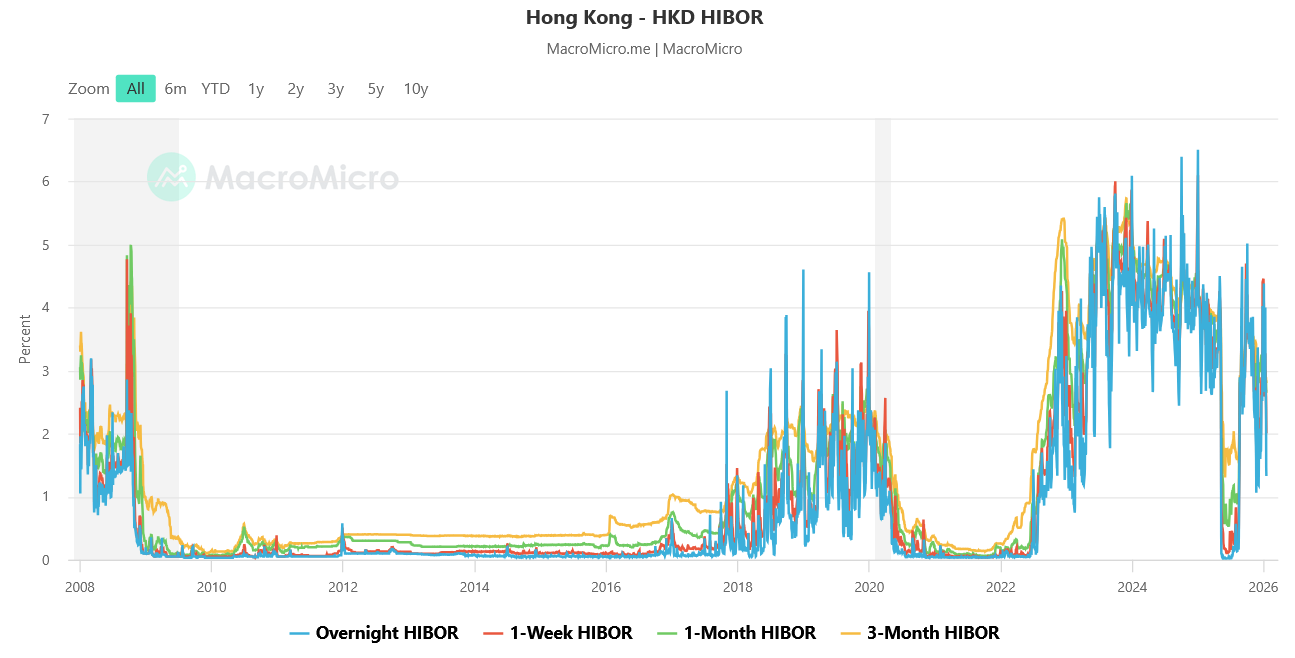
\includegraphics[width=\textwidth,height=0.55\textheight,keepaspectratio]{figures/slide15_img_flat.png}
\end{column}
\begin{column}{0.5\textwidth}
\centering
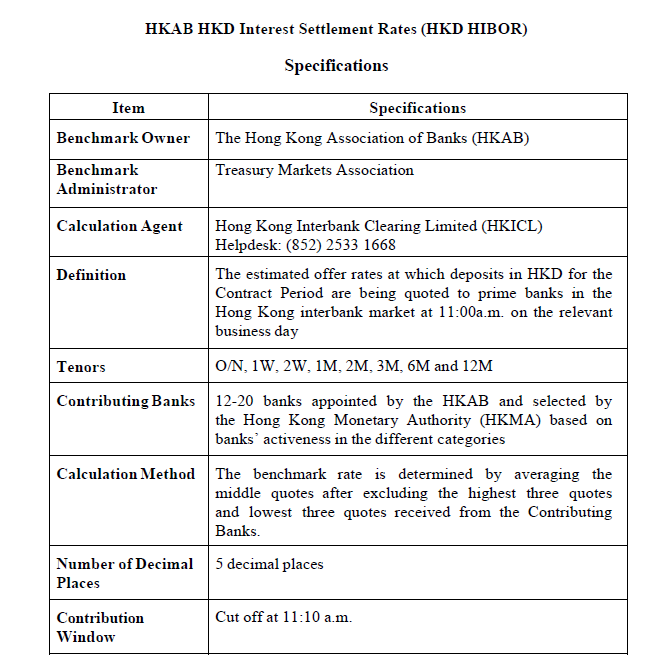
\includegraphics[width=\textwidth,height=0.55\textheight,keepaspectratio]{figures/slide16_img_flat.png}
\end{column}
\end{columns}
\end{frame}

% [src: 17]
\begin{frame}{What Shifts the Curves? Supply-Side Factors}
\begin{table}
\centering
\small
\begin{tabular}{p{0.2\textwidth}p{0.1\textwidth}p{0.58\textwidth}}
\toprule
\textbf{Increase in} & \textbf{Supply} & \textbf{Why / Result} \\
\midrule
Wealth \& income & $\uparrow$ & More funds available for investment --- \emph{lower} interest rate \\
Risk & $\downarrow$ & Riskier securities are less attractive to fund suppliers --- \emph{higher} rate \\
Near-term spending needs & $\downarrow$ & Fewer funds available to invest --- \emph{higher} rate \\
Monetary expansion & $\uparrow$ & Central-bank money creation directly increases lendable funds --- \emph{lower} rate \\
\bottomrule
\end{tabular}
\end{table}
\note{Increase in wealth increases the supply of loanable funds because the marginal propensity to consume decreases with wealth.}
\end{frame}

% [src: 18]
\begin{frame}{What Shifts the Curves? Factors Moving Both Sides}
\begin{table}
\centering
\small
\begin{tabular}{p{0.19\textwidth}p{0.1\textwidth}p{0.1\textwidth}p{0.49\textwidth}}
\toprule
\textbf{Increase in} & \textbf{Supply} & \textbf{Demand} & \textbf{Why / Result} \\
\midrule
Economic growth & $\uparrow$ & $\uparrow$ & Wealth and income rise (more supply); more projects profitable (more demand) --- effect on rate \emph{indeterminate} \\
Utility from assets & $\downarrow$ & $\uparrow$ & Suppliers less willing to save; demanders more willing to borrow --- \emph{higher} rate \\
Restrictive covenants & $\uparrow$ & $\downarrow$ & Borrowers demand less; lenders more willing to supply --- \emph{lower} rate \\
Tax rate & $\downarrow$ & $\uparrow$ & Taxes reduce after-tax returns to savers; interest deductibility raises borrowing demand --- \emph{higher} rate \\
\bottomrule
\end{tabular}
\end{table}
\end{frame}

% [src: 19]
\begin{frame}{Case: The Global Savings Glut}
\begin{quote}
``Whether it was a glut of excess intended saving, or a shortfall of investment intentions, the result was the same: a fall in global real long-term interest rates and their associated capitalization rates. Asset prices, particularly house prices, in nearly two dozen countries accordingly moved dramatically higher.'' --- Alan Greenspan, 2010
\end{quote}
\begin{center}

\includegraphics[height=0.46\textheight,keepaspectratio]{figures/slide19_img.jpg}
\end{center}
\note{Alan Greenspan served as Chairman of the Federal Reserve of the United States from 1987 to 2006.}
\end{frame}

% [src: 20]
\begin{frame}{Determinants of Rates for Individual Securities}
\begin{equation*}
i_j^* = f(IP,\ RFR,\ DRP_j,\ LRP_j,\ SCP_j,\ MP_j)
\end{equation*}
where $i_j^*$ = equilibrium nominal interest rate for security $j$.
\begin{description}
  \item[Inflation premium (IP)] $IP = \frac{CPI_{t+1} - CPI_t}{CPI_t} \times 100$; CPI = price level of a basket of goods and services purchased by the typical urban consumer
  \item[Real risk-free rate (RFR)] $RFR = i - E(IP)$; measures society's relative time preference for consuming today rather than tomorrow
\end{description}
\note{The exact Fisher effect: $(1+i) = (1+RFR)(1+E(IP))$, i.e., $i = RFR + E(IP) + RFR \cdot E(IP)$.}
\end{frame}

% [src: 21]
\begin{frame}{Default Risk Premium (DRP)}
Compensation for the risk that the issuer fails to pay:
\begin{equation*}
DRP_j = i_{jt} - i_{Tt}
\end{equation*}
where $i_{jt}$ = interest rate on security $j$ at time $t$ and $i_{Tt}$ = rate on a similar-maturity U.S.\ Treasury security at time $t$.
\begin{center}
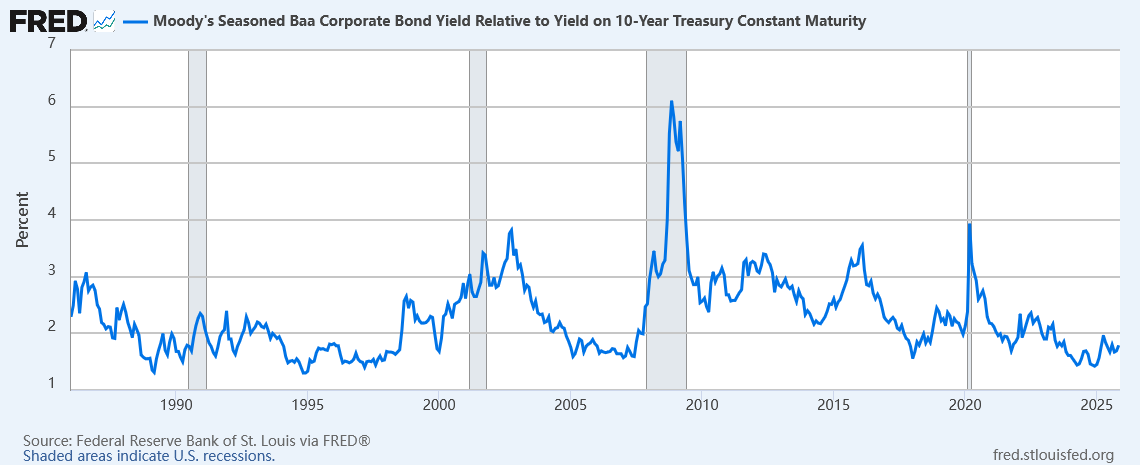
\includegraphics[height=0.46\textheight,keepaspectratio]{figures/slide21_img_flat.png}
\end{center}
\note{DRPs are compensation for default risk, are countercyclical, and rise in periods of weak economic conditions.}
\end{frame}

% [src: 22]
\begin{frame}{Remaining Security-Specific Premiums}
\begin{description}
  \item[Liquidity risk premium (LRP)] Extra required yield to offset the risk of not being able to sell the asset in a timely fashion at fair value
  \item[Special feature premium (SCP)] Taxability (municipal bonds exempt from federal/state taxes); convertibility (convertible bonds have lower yields); callability (callable bonds require higher yields)
  \item[Maturity premium (MP)] Difference between yields on long- and short-term securities of the same characteristics
\end{description}
\vspace{0.3em}
Inflation and the real risk-free rate are the \textbf{same for all securities}; DRP, LRP, SCP, and MP are \textbf{security-specific}.
\note{Convertible bond: the bondholder has the right to convert into preferred or common stock at their choice. Callable bond: the issuer has the right to call back the bond at a pre-determined price.}
\end{frame}

% ============ PART II: TERM STRUCTURE ============

% [src: 23]
\section{Term Structure of Interest Rates}

% [src: 24]
\begin{frame}{Term Structure of Interest Rates (Yield Curve)}
The \textbf{term structure of interest rates} (also called the \textbf{yield curve}) describes the relationship between interest rates (yields) and different maturities for bonds of similar credit quality (typically government bonds).
\vspace{0.4em}
Typical shapes, plotting yield to maturity against time to maturity:
\begin{description}
  \item[(a) Upward sloping] yields rise with maturity (``normal'')
  \item[(b) Inverted / downward sloping] yields fall with maturity
  \item[(c) Flat] yields roughly equal across maturities
\end{description}
\note{The shape of the term structure of interest rates is also called the ``yield curve.''}
\end{frame}

% [src: 25]
\begin{frame}{Three Theories of the Term Structure}
Several major theories explain why the yield curve takes different shapes --- upward-sloping (normal), flat, downward-sloping (inverted), or humped --- and what drives long-term vs.\ short-term rates:
\begin{description}
  \item[Unbiased expectations theory (UET)] Long-term rates are purely the geometric average of current and expected future short-term rates
  \item[Liquidity premium theory] Builds on pure expectations but adds a positive liquidity (term) premium that increases with maturity
  \item[Market segmentation theory] Markets for different maturities are completely separate; investors and borrowers have strict maturity preferences and do not substitute across maturities
\end{description}
\end{frame}

% [src: 26, 27]
\begin{frame}{Unbiased Expectations Theory (UET)}
Long-term rates are geometric averages of current and expected future short-term rates:
\begin{equation*}
{}_1R_N = \left[(1+{}_1R_1)(1+E({}_2r_1)) \cdots (1+E({}_Nr_1))\right]^{1/N} - 1
\end{equation*}
with ${}_1R_N$ = annualized rate on an $N$-year bond, ${}_1R_1$ = actual one-year rate today, and $E({}_ir_1)$ = expected one-year rate from year $i-1$ to $i$.
\vspace{0.3em}

UET is a good benchmark: in equilibrium, the return from holding an $N$-year bond to maturity should equal the expected return from investing in $N$ successive one-year bonds.
% Source slide 26/27 formula images (slide26_img.png, slide27_img.png) dropped: equations typeset natively above.
\note{Assumes no interest-rate volatility; these rates are zero-coupon (``spot'') rates.}
\end{frame}

% [src: 28]
\begin{frame}{Constructing a Yield Curve with UET: Example}
Suppose the current one-year rate and expected one-year rates are ${}_1R_1 = 1.94\%$, $E({}_2r_1) = 3\%$, $E({}_3r_1) = 3.74\%$, $E({}_4r_1) = 4.10\%$. Under UET, today's one-, two-, three-, and four-year Treasury rates are ${}_1R_1 = 1.94\%$ and:
\begin{center}
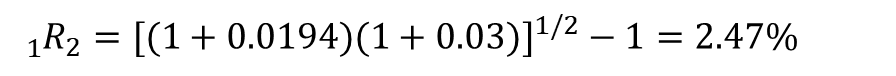
\includegraphics[width=0.31\textwidth,keepaspectratio]{figures/slide28_img_flat.png}
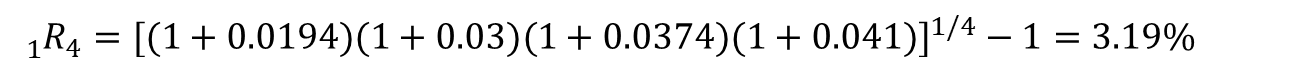
\includegraphics[width=0.31\textwidth,keepaspectratio]{figures/slide28_img1_flat.png}
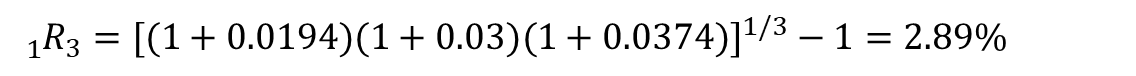
\includegraphics[width=0.31\textwidth,keepaspectratio]{figures/slide28_img2_flat.png}
\end{center}
\note{The 2-year maturity rate is the geometric average of the current 1-year rate and the expected 1-year rate prevailing in the second year.}
\end{frame}

% [src: 29]
\begin{frame}{Liquidity Premium Theory}
Long-term rates are geometric averages of current and expected future short rates \emph{plus a liquidity premium that increases with maturity}:
\begin{equation*}
{}_1R_N = \left[(1+{}_1R_1)(1+E({}_2r_1)) \cdots (1+E({}_Nr_1)) + L_N\right]^{1/N} - 1
\end{equation*}
where $L_t$ = liquidity premium for period $t$, with $L_2 < L_3 < \cdots < L_N$.
\vspace{0.3em}

The theory implicitly assumes investors prefer short-term securities --- more liquid, and prices less sensitive to interest-rate changes.
% Source slide 29 formula image (slide29_img.png) dropped: equation typeset natively above.
\end{frame}

% [src: 30]
\begin{frame}{UET vs.\ Liquidity Premium Theory}
\begin{figure}
\centering
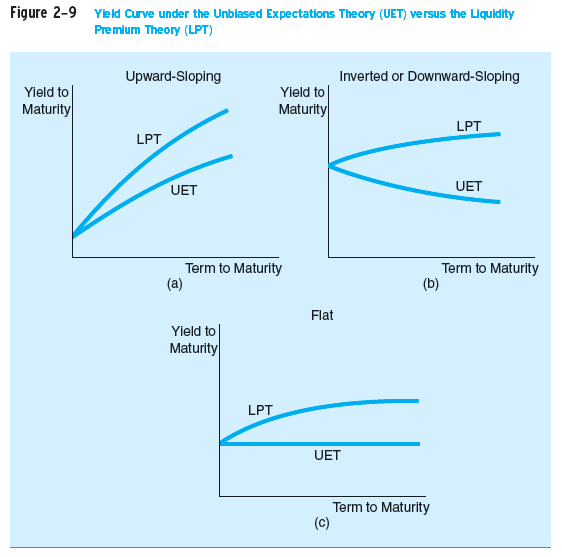
\includegraphics[height=0.70\textheight,keepaspectratio]{figures/slide30_img.png}
\end{figure}
\end{frame}

% [src: 31]
\begin{frame}{Market Segmentation Theory}
Investors and financial institutions have \textbf{specific maturity preferences}:
\begin{itemize}
  \item Money market funds prefer short-term Treasury bonds
  \item Insurance companies and pension funds prefer longer-maturity bonds
\end{itemize}
\vspace{0.3em}
Yields in each maturity segment are determined \emph{independently} by supply and demand within that segment; investors and borrowers deviate from their preferred segment only when adequately compensated. Under this theory, the long-term rate is \textbf{unrelated} to expected future short-term rates.
\end{frame}

% [src: 32]
\begin{frame}{Comparison Between Theories}
\begin{table}
\centering
\small
\begin{tabular}{p{0.17\textwidth}p{0.19\textwidth}p{0.17\textwidth}p{0.14\textwidth}p{0.17\textwidth}}
\toprule
\textbf{Theory} & \textbf{Key Driver} & \textbf{Risk/Term Premium?} & \textbf{Typical Bias} & \textbf{Best Explains\ldots} \\
\midrule
Unbiased expectations & Expectations of future short rates & None & Any shape (no bias) & Changes in curve shape over time \\
Liquidity premium & Expectations + liquidity premium & Positive \& increasing with maturity & Upward & Persistent upward slope historically \\
Segmented markets & Supply \& demand in maturity segments & Independent per segment & Any shape & Supply/demand-driven anomalies \\
\bottomrule
\end{tabular}
\end{table}
\end{frame}

% [src: 33]
\begin{frame}{Yield Curve Shapes: Stylized Analysis}
\begin{table}
\centering
\small
\begin{tabular}{p{0.22\textwidth}p{0.16\textwidth}p{0.16\textwidth}p{0.22\textwidth}}
\toprule
\textbf{Characteristic} & \textbf{Early 2021 (Normal)} & \textbf{Jul 2023 (Inverted)} & \textbf{Sep 2026 (Normal, flat)} \\
\midrule
3M yield & $\sim$0.05\% & $\sim$5.30\% & $\sim$3.87\% \\
10Y yield & $\sim$1.00\% & $\sim$3.96\% & $\sim$4.79\% \\
Slope (10Y$-$3M) & $+$\,$\sim$95bp & $\sim$$-$134bp & $+$\,$\sim$92bp \\
Signal & Expansion & Recession fear & Expansion (flat curve) \\
\bottomrule
\end{tabular}
\end{table}
\vspace{0.2em}
\begin{center}
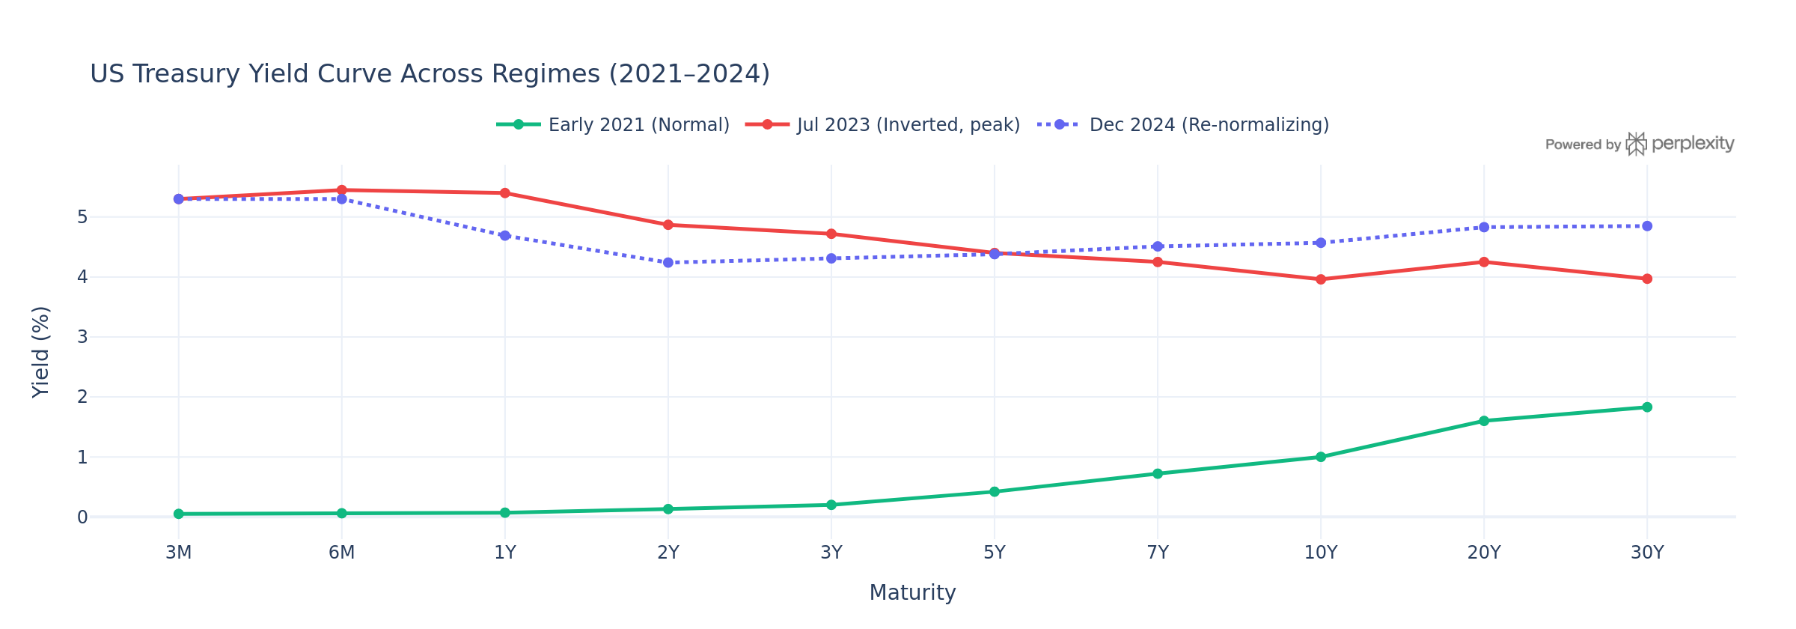
\includegraphics[width=0.9\textwidth,height=0.36\textheight,keepaspectratio]{figures/slide33_img_flat.png}
\end{center}
\note{You can check out the US Treasuries yield curve on the Treasury's website: \href{https://www.ustreasuryyieldcurve.com/}{ustreasuryyieldcurve.com}.}
\end{frame}

% [src: 34]
\begin{frame}{US Treasury Yield Curve}
\begin{figure}
\centering
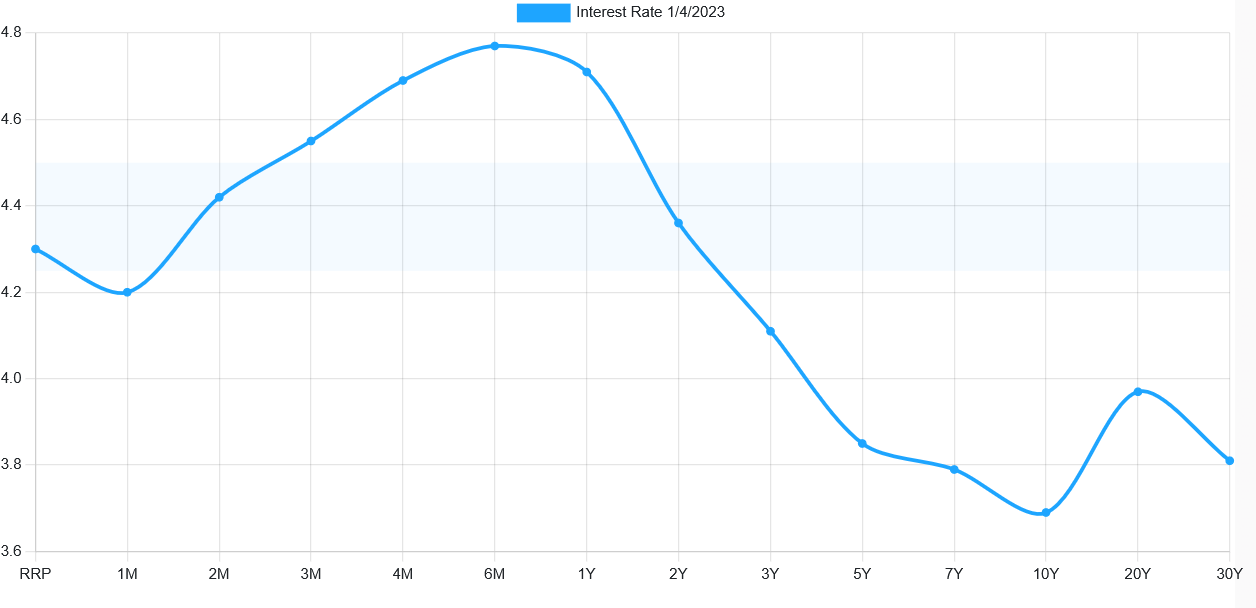
\includegraphics[height=0.75\textheight,keepaspectratio]{figures/slide34_img_flat.png}
\end{figure}
\end{frame}

% [src: 35]
\begin{frame}{Government Bond Yield Curves in Other Markets}
\begin{columns}
\begin{column}{0.5\textwidth}
\centering

\includegraphics[width=\textwidth,keepaspectratio]{figures/slide35_img.png}
\end{column}
\begin{column}{0.5\textwidth}
\centering
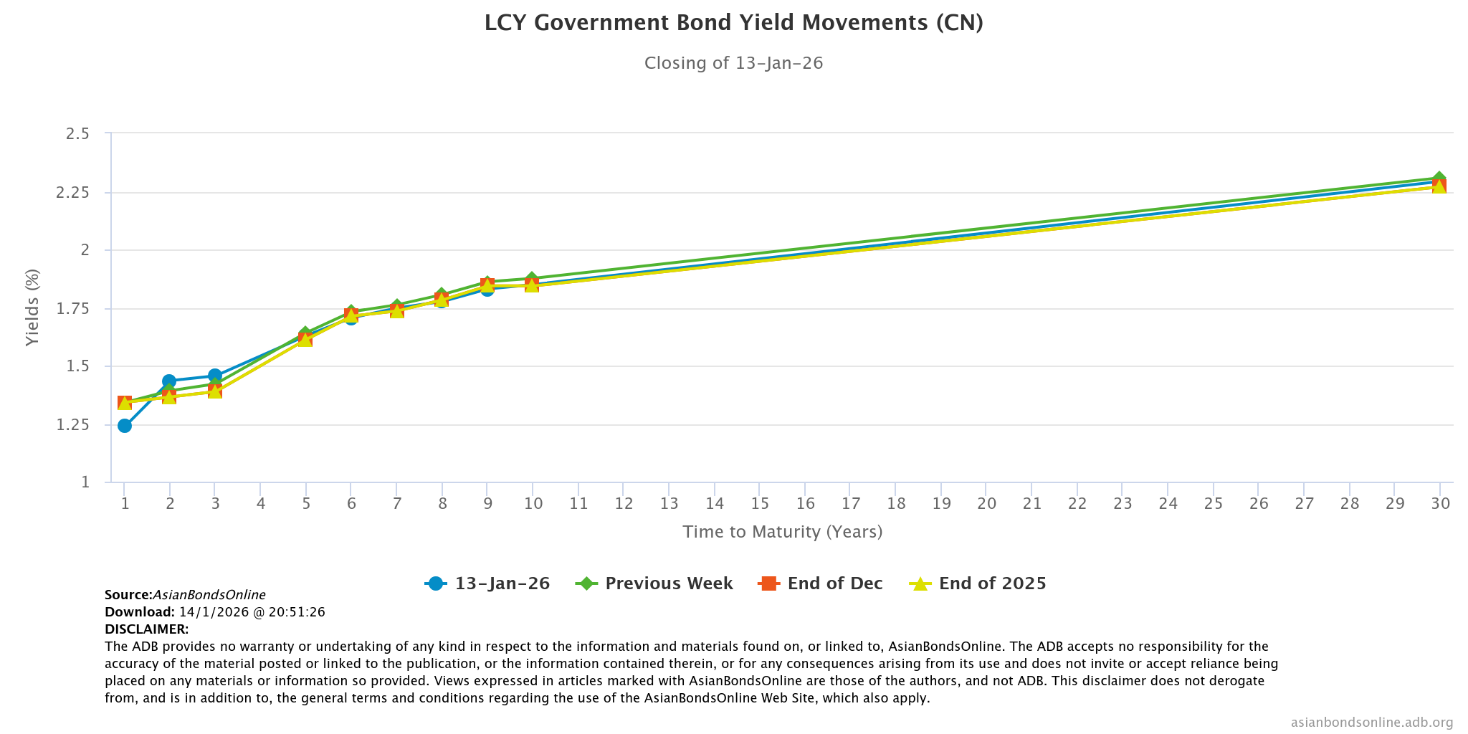
\includegraphics[width=\textwidth,keepaspectratio]{figures/slide35_img1.png}
\end{column}
\end{columns}
\vspace{0.2em}
\begin{center}
\small Source: \href{https://asianbondsonline.adb.org/market-watch/}{asianbondsonline.adb.org}
\end{center}
\end{frame}

% [src: 36]
\begin{frame}{Implied Forward Rates}
A \textbf{forward rate} ($f$) is an expected rate on a short-term bond to be originated at some point in the future. UET states
\begin{equation*}
(1+{}_1R_N)^N = (1+{}_1R_1)(1+E({}_2r_1))\cdots(1+E({}_Nr_1))
\end{equation*}
Rearranging for adjacent maturities gives the one-year forward rate from year $N-1$ to year $N$:
\begin{equation*}
{}_{N-1}f_1 = \frac{(1+{}_1R_N)^{N}}{(1+{}_1R_{N-1})^{N-1}} - 1
\end{equation*}
% Source slide 36 formula images (slide36_img*.png) dropped: equations typeset natively above.
\note{If UET strictly holds, forward rates are an unbiased estimate of expected future short rates. If there are liquidity premiums, subtract the liquidity premium from the forward rate before using it as an estimate of the expected future spot rate. If segmentation strictly holds, the forward rate has no economic meaning.}
\end{frame}

% [src: 37]
\begin{frame}{Implied Forward Rates: Example}
Suppose (illustrative numbers, in the spirit of the low-rate 2010s) the spot one-, two-, three-, and four-year zero-coupon Treasury rates are ${}_1R_1 = 0.156\%$, ${}_1R_2 = 0.305\%$, ${}_1R_3 = 0.499\%$, ${}_1R_4 = 0.753\%$. Using UET, the one-year forward rates from year 1 to 2, 2 to 3, and 3 to 4 are:
\begin{center}

\includegraphics[width=0.31\textwidth,keepaspectratio]{figures/slide37_img_flat.png}

\includegraphics[width=0.31\textwidth,keepaspectratio]{figures/slide37_img1_flat.png}
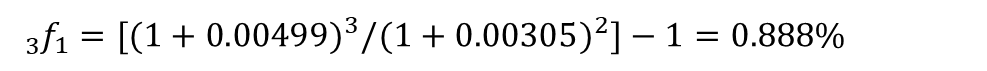
\includegraphics[width=0.31\textwidth,keepaspectratio]{figures/slide37_img2_flat.png}
\end{center}
\end{frame}

% [src: 38]
\begin{frame}{The Yield Curve Inverts Before Recessions}
Spread: 5-year Treasury note minus 3-month Treasury bill.
\begin{figure}
\centering
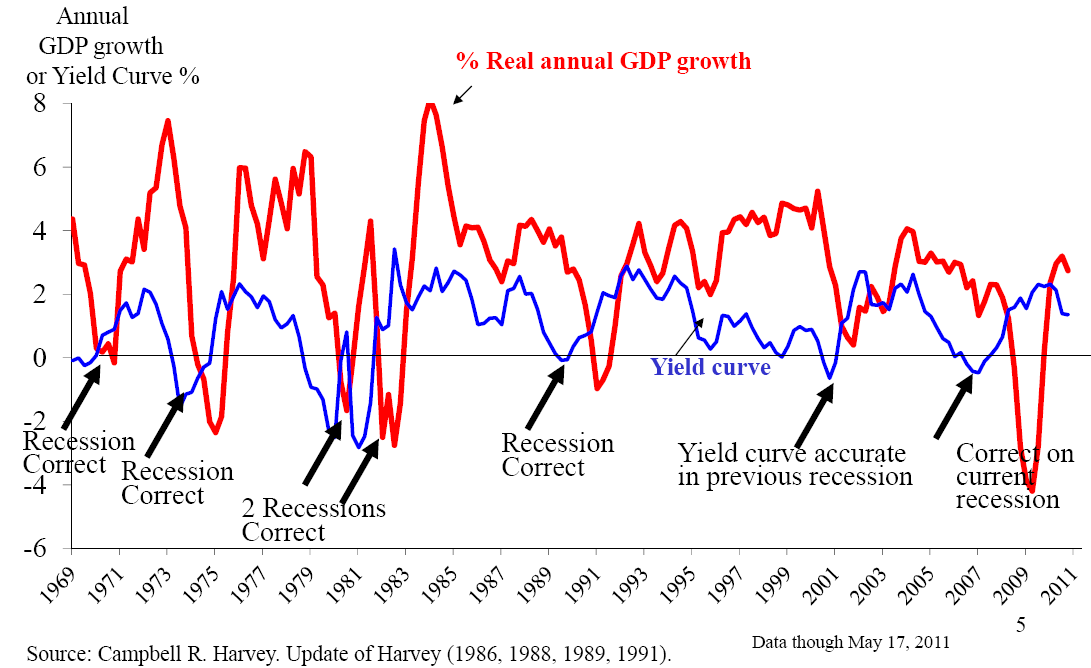
\includegraphics[height=0.66\textheight,keepaspectratio]{figures/slide38_img.png}
\end{figure}
\begin{center}
\small Source: \href{http://www.duke.edu/~charvey/research_term_structure.htm}{duke.edu/\textasciitilde charvey}
\end{center}
\note{Related: \href{https://www.researchaffiliates.com/en_us/insights/conversations/flattening-yield-curve.html}{researchaffiliates.com --- flattening yield curve}.}
\end{frame}

% [src: 39, 40]
\begin{frame}{Mechanisms Behind the Predictability}
\textbf{Main mechanism --- expectations of future Fed rate cuts due to economic weakness.} Bond markets price Treasuries off expected future short rates (heavily influenced by the federal funds rate) plus a term premium for risk and inflation uncertainty.
\begin{itemize}
  \item Upward-sloping curve: investors expect short rates to rise (or stay stable) --- typical of expansions
  \item Inverted curve: investors expect short rates to fall significantly --- usually because they anticipate slowdown or recession
\end{itemize}
\vspace{0.3em}
\textbf{Secondary channel --- tight policy and credit conditions.} Inversions often follow aggressive Fed hikes: short yields jump while long yields rise less (or fall) on expected easing. Tightening slows the economy by raising borrowing costs and squeezing bank net interest margins (borrow short, lend long), leading banks to tighten lending standards; reduced credit amplifies weakness.
\end{frame}

% [src: 41]
\begin{frame}{But the Signal Gave a False Alarm Recently\ldots}
The long 2022--2024 inversion was the longest on record and was not followed by an immediate recession, leading some to question its reliability --- but the core logic still holds in most analyses. The curve has since returned to a normal shape: as of September 2026 it is positively sloped but unusually flat (10Y exceeds 2Y by only $\sim$40\,bp).
\begin{center}
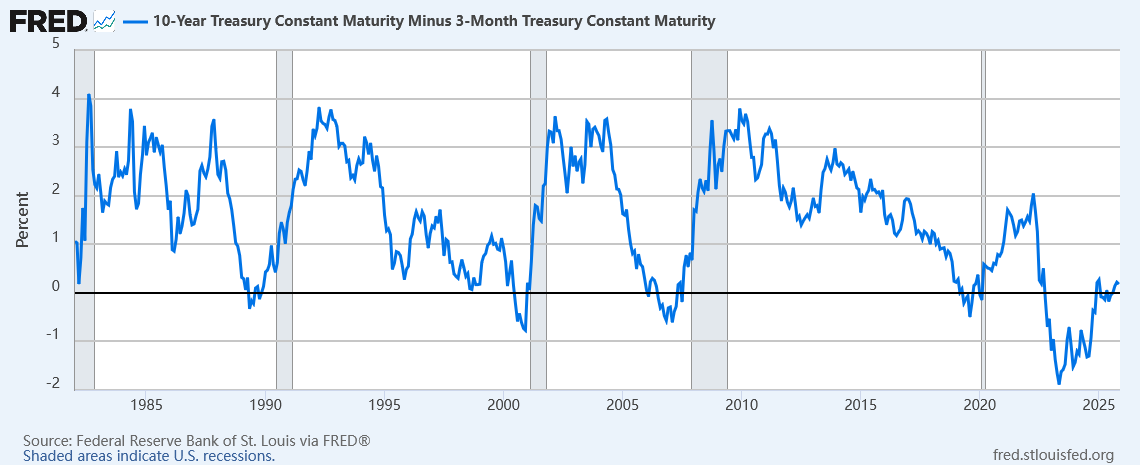
\includegraphics[height=0.52\textheight,keepaspectratio]{figures/slide41_img_flat.png}
\end{center}
\begin{center}
\small Source: \href{https://fred.stlouisfed.org/series/T10Y3M}{FRED, T10Y3M}
\end{center}
\end{frame}

% ============ PART III: TIME VALUE OF MONEY ============

% [src: 42]
\section{Time Value of Money}

% [src: 43, 44, 45]
\begin{frame}{Time Value of Money: Lump Sums}
A dollar received today is worth more than a dollar received in the future. \textbf{Simple interest}: interest is not reinvested. \textbf{Compound interest}: interest is reinvested (the standard assumption in finance).
\begin{description}
  \item[Present value] Discount a future payment at the current rate:
    $PV = FV_t\left[\frac{1}{1+r}\right]^{t} = FV_t \cdot PVIF_{r,t}$
  \item[Future value] Compound a present sum:
    $FV_t = PV(1+r)^{t} = PV \cdot FVIF_{r,t}$
\end{description}
\vspace{0.2em}
where $FV_t$ = future lump sum received in $t$ periods, $r$ = annual interest rate, $t$ = years, and $PVIF_{r,t}$ ($FVIF_{r,t}$) = present (future) value interest factor of a lump sum.
\end{frame}

% [src: 46]
\begin{frame}{Present Value of an Annuity}
The present value of a finite series of equal cash flows received at the \emph{end} of each equal interval (ordinary annuity):
\begin{equation*}
PV = PMT \cdot PVIFA_{r,t}, \qquad PVIFA_{r,t} = \sum_{n=1}^{t} \frac{1}{(1+r)^{n}}
\end{equation*}
If cash flows arrive on the \emph{first} day of each period (annuity due), each payment earns one extra period of interest:
\begin{equation*}
PV^{due} = PMT \cdot PVIFA_{r,t} \times (1+r)
\end{equation*}
% Source slide 46 formula images (slide46_img*.png) dropped: equations typeset natively above.
\note{Note that $1/(1+i)^N = (1+i)^{-N}$.}
\end{frame}

% [src: 47]
\begin{frame}{Present Value of an Annuity: Example}
A bond pays \$10,000 on the last day of every year for the next six years, in exchange for a fixed payment today. At an annual rate of 8\%:
\begin{center}
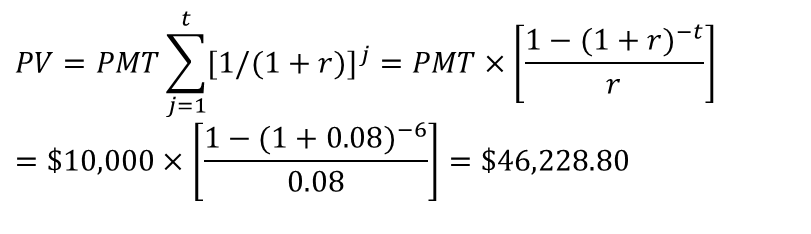
\includegraphics[width=0.4\textwidth,keepaspectratio]{figures/slide47_img_flat.png}
\end{center}
If instead it pays \$10,000 on the last day of every \emph{quarter} for six years ($r = 8\%/4 = 2\%$, $t = 6\times4 = 24$), the present value becomes:
\begin{center}
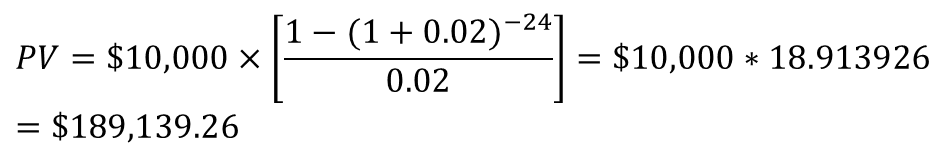
\includegraphics[width=0.4\textwidth,keepaspectratio]{figures/slide47_img1_flat.png}
\end{center}
\note{Note that $1/(1+i)^N = (1+i)^{-N}$.}
\end{frame}

% [src: 48]
\begin{frame}{Future Value of an Annuity}
The future value of a finite series of equal cash flows received at the end of each interval:
\begin{equation*}
FV_t = PMT \cdot FVIFA_{r,t}, \qquad FVIFA_{r,t} = \sum_{n=1}^{t}(1+r)^{t-n} = \frac{(1+r)^{t}-1}{r}
\end{equation*}
% Source slide 48 formula image (slide48_img.png) dropped: equation typeset natively above.
\end{frame}

% [src: 49]
\begin{frame}{Future Value of an Annuity: Example}
You want \$5 million when you retire in 40 years and believe you can earn 9\% per year. How much must you invest each year, with the first investment at the end of the first year? (Ignore taxes.)
\begin{center}

\includegraphics[width=0.55\textwidth,keepaspectratio]{figures/slide49_img_flat.png}
\end{center}
\begin{center}
$PMT = \$14{,}798$
\end{center}
\end{frame}

% [src: 50]
\begin{frame}{Key Takeaways}
\begin{description}
  \item[Determinants of interest rates] Real risk-free rate + inflation expectations (Fisher effect: $i \approx RFR + E(IP)$); market equilibrium set by supply (savings) and demand (borrowing) of loanable funds; security-specific yields add premiums for default, liquidity, maturity, and special features
  \item[Term structure (yield curve)] Relationship between yield and maturity for similar-risk bonds; theories --- expectations (long rates = average of expected future short rates), liquidity premium (extra compensation for longer maturities), market segmentation (supply and demand within maturity segments set rates independently)
  \item[Key insight] An inverted curve signals expected rate cuts and predicts recession
\end{description}
\end{frame}

% ============ GROUP PROJECT RUBRICS ============

% [src: 51]
\section{Group Project Grading Rubrics}

% [src: 52]
\begin{frame}{Grading Rubrics: Four Dimensions}
\begin{table}
\centering
\small
\begin{tabular}{p{0.32\textwidth}p{0.13\textwidth}p{0.15\textwidth}p{0.13\textwidth}p{0.13\textwidth}}
\toprule
\multicolumn{5}{l}{\textit{Presentation (10 points)}} \\
\midrule
Content and Ideas (4) & Poor (60\%) & Satisfactory (75\%) & Good (85\%) & V.\ Good (95\%) \\
Effective Use of Resources (2) &  &  &  &  \\
Creativity/Novelty (2) &  &  &  &  \\
Presentation Skill (2) &  &  &  &  \\
\midrule
\multicolumn{5}{l}{\textit{Report (20 points)}} \\
\midrule
Content and Ideas (8) & Poor (60\%) & Satisfactory (75\%) & Good (85\%) & V.\ Good (95\%) \\
Effective Use of Resources (4) &  &  &  &  \\
Creativity/Novelty (4) &  &  &  &  \\
Writing Clarity (4) &  &  &  &  \\
\bottomrule
\end{tabular}
\end{table}
\end{frame}

% [src: 53, 54]
\begin{frame}{Grading Rubrics Explained}
\begin{description}
  \item[1. Content and ideas] The foundational substance and intellectual core --- not just information, but a purposeful, insightful, well-structured argument or exploration
  \item[2. Effective use of resources] How you select, integrate, and build on existing evidence --- use authoritative, relevant sources (scholarly articles, reputable books, reliable data, primary sources); avoid weak sources such as unexplained web pages or popular forums
  \item[3. Creativity / novelty] The unique perspective, innovative approach, or original contribution --- ask your group: ``What will make our project memorable and distinct from seven other groups doing a similar topic?''
  \item[4. Writing clarity and presentation] The precision, polish, and professionalism of the communication --- does the final product read as one unified voice? Seamless integration of different writers' sections is crucial
\end{description}
\end{frame}

\end{document}
